\documentclass{article}
\usepackage{polski}
\usepackage{blindtext}
\usepackage{amsmath}
\usepackage{mathtools}
\usepackage{graphicx} 
\usepackage{wrapfig}
\usepackage{amssymb}
\usepackage{multirow}
\usepackage[usenames,dvipsnames,svgnames,table]{xcolor}
\usepackage{float}
\usepackage[caption = false]{subfig}
\usepackage{caption}
\newcommand\tab[1][1cm]{\hspace*{#1}}
\usepackage[a4paper, left=2cm, right=2cm, top=2cm, bottom=2cm, headsep=1.2cm]{geometry}

\usepackage{titling}
\newcommand{\subtitle}[1]{%
  \posttitle{%
    \par\end{center}
    \begin{center}\large#1\end{center}
    \vskip0.5em}%
}


\begin{document}
\title{Poszukiwanie minimum wartości funkcji metodą największego spadku
w 2D}
\author{Wiktoria Zaczyk}
\date{13.05.2021}

\maketitle	


\section{Wstęp}

\textbf{Minimalizacja funkcji}
\newline
Inaczej nazywana optymalizacją, jej zadaniem jest poszukiwanie odpowiednio minimum lub maksimum funkcji wielu zmiennych. Chodzi o znalezienie punktu spełniającego warunek
\begin{equation}
\min f(\vec{x}) = f(\vec{x^{*}}) \Leftrightarrow \bigwedge_{\vec{x} \in R^n} f(\vec{x^{*}}) < f(\vec{x}), \quad \text{ gdzie } \vec{x} = [x_1, x_2, \dots, x_n]^{T}.
\end{equation}
\textbf{Gradient funkcji}
\newline
Dla funkcji celu $f(\vec{x}) \in C^2$, tj. poszukującej minimum badanej funkcji wejściowej definiuje się funkcję wektorową będącą gradientem funkcji
\begin{equation}
g(\vec{x}) = \nabla f(\vec{x}) = \bigg[ \frac{\partial f(\vec{x})}{\partial x_1}, \frac{\partial f(\vec{x})}{\partial x_2}, \dots, \frac{\partial f(\vec{x})}{\partial x_n}, \bigg]^{T}.
\end{equation}
Należy pamiętać, iż gradient skierowany jest zawsze w stronę narastających wartości.
\newline\newline
\textbf{Pochodna kierunkowa funkcji celu}
\newline
Różniczkę zupełną funkcji celu definiuje się jako iloczyn skalarny wektorów
\begin{equation}
df = \frac{\partial f}{\partial x_1} dx_1 +  \cdots + \frac{\partial f}{\partial x_n} dx_n = \nabla f(\vec{x}) dx.
\end{equation}
Punkty  $\vec{x}$ i $\vec{x'}$ nazywane są powiązanymi ze sobą, jeżeli wektor $\vec{u}$ wyznacza kierunek prostej je łączącej, stąd
\begin{equation}
\vec{x}(\lambda) = \vec{x'} + \lambda \vec{u} .
\label{lambda}
\end{equation}
Dla bardzo małych zmian wartości $\lambda$ można uogólnić wzór (\ref{lambda}).
\begin{equation}
d\vec{x} = \vec{u} d\lambda
\end{equation}
Na prostej łączacej ustalone punkty $\vec{x}$ oraz $\vec{x'}$ wartość funkcji celu zależna jest od zmiennej $\lambda$.
\begin{equation}
F(\lambda) = f(\vec{x'} + \lambda \vec{u} ) = f(\vec{x})
\end{equation}
Mając na uwadze powyższe powiązania, oblicza się różniczkę zupełną dla funkcji celu zależnej od $\lambda$
\begin{equation}
dF = df = \nabla^{T} f(\vec{x}) \vec{u} d \lambda.
\end{equation}
Finalnie, wyrażenie na \textbf{pochodną kierunkową funkcji} celu w punkcie $\vec{x}$ dla kierunku $\vec{u}$ jest postaci
\begin{equation}
\frac{d F (\lambda)}{d\lambda} = \left.\frac{df(\vec{x})}{d\lambda}\right|_{\vec{u}} = \nabla^{T} f(\vec{x}) \vec{u}, 
\label{wzor}
\end{equation}
jednak korzystając z niej należy ją wyznaczać w każdej iteracji.
\newline\newline
\textbf{Znajdowanie minimum funkcji przy pomocy pochodnej kierunkowej}
\newline
Przybliżanie należy rozpocząć z punktu $\vec{x_0}$ przechodząc przez kolejne punkty $\vec{x_1}, \vec{x_2}, \dots, \vec{x_n}$ w kierunku spadku wartości funkcji. Pozwala to wyznaczyć ciąg przybliżeń poszukiwanego minimum. Należy przerwać algorytm iteracyjny w momencie, gdy zostanie spełniony jeden z warunków:
\begin{enumerate}
	 \item Norma różnicy wektorów z sąsiednich kroków jest mniejsza od zadanego progu: $||\vec{x}^{i+1} - \vec{x}^i|| < \epsilon$
	 $\nabla f(\vec{x}) = 0$
	 \item W kolejnych iteracjach wartość normy $||\vec{x}^{i+1} - \vec{x}^i||$ wzrasta, co oznacza brak zbieżności.
\end{enumerate}
\textbf{Metoda największego spadku}
\newline
Korzystając z pochodnej kierunkowej funkcji w punkcie x dla wektora kierunkowego $\vec{u}$ o długości równej $||\vec{u}|| = 1$
	\begin{equation}
	\left.\frac{\text{d}f(\vec{x'})}{\text{d}\lambda}\right|_{\vec{u}} = \frac{\text{d}F(0)}{\text{d}\lambda} = 
	\nabla ^{T} f(\vec{x'})\vec{u},
	\end{equation}
oraz z nierówność Schwartza \begin{equation}
	\nabla^{T} f(\vec{x'}) \vec{u} \geq - ||\nabla^{T} f(\vec{x'})|| \cdot || \vec{u}  || = 
	- || \nabla ^{T} f(\vec{x'})|| = \min.
	\end{equation}
Należy wybrać wektor kierunkowy o postaci
\begin{equation}
\vec{u} = \frac{- \nabla f(\vec{x'})}{||\nabla f(\vec{x'})||}
\end{equation}
aby wskazywał kierunek największego spadku, a pochodna kierunkowa mogła osiągnąć najmniejszą wartość.
\begin{equation}
\frac{\text{d} F(0) }{\text{d} \lambda} = - \nabla^T f(\vec{x'})  \frac{\nabla f(\vec{x'})}{||\nabla f(\vec{x'})||} = \min
\end{equation}

\section{Cel zadania}

Celem laboratorium było znalezienie minimum przy pomocy metody największego spadku w 2D funkcji:
\begin{equation}
f(\vec{r}) =  f(x, y) = \frac{5}{2} (x^2 - y)^2 + (1 - x )^2,
\label{lol}
\end{equation}
zaczynając od przybliżenia $\vec{r_0}$:
\begin{equation}
\vec{r_{i+1}} = \vec{r_i} - h\cdot\nabla \left.f(\vec{r})\right|_{\vec{r} = \vec{r_i}} \quad \text{ gdzie } \nabla f(\vec{r}) = \left[\frac{\partial f}{\partial x}, \frac{\partial f}{\partial y}\right],
\label{15}
\end{equation}
które było korygowane w kolejnych iteracjach.
Składowe gradientu ze wzoru (\ref{15}) obliczano numerycznie korzystając z faktu, iż
\begin{equation}
\frac{\partial f(\vec{r})}{\partial  x} = \frac{f(\vec{r} + \Delta \vec{e_x}) - f(\vec{r} - \Delta \vec{e_x})}{2 \Delta}
\end{equation}
\begin{equation}
\frac{\partial f(\vec{r})}{\partial  y} = \frac{f(\vec{r} + \Delta \vec{e_y}) - f(\vec{r} - \Delta \vec{e_y})}{2 \Delta}
\end{equation}
gdzie $\vec{e_x}$ i $\vec{e_y}$ są wektorami układu kartezjańskiego.
Przyjęto następujące założenia:
$\Delta = 10^{-4}$, punkt początkowy $\vec{r_0} = [-0.75, 1.75]$, stała $h = 0.01$. Warunki stopu:
$||\vec{r_{i+1}} - \vec{r_i}||_2 < \epsilon$ dla $\epsilon_1 = 10^{-2}$, $\epsilon_2 = 10^{-3}$
Maksymalna liczba iteracji 1000, a 
$x, y \in [-2, 2]$ z krokiem w obu kierunkach równym 0.02
\newpage
\section{Wyniki}

Korzystając skryptu programu \textit{Gnuplot} sporządzono wykresy dla obu przypadków. Dokładne minimum funkcji było jedno i wyniosło $\vec{r}_m_i_n=[1,1]$ (zaznaczone czarnym krzyżykiem). Na rysunkach znajdują się także kontur wartości funkcji $ f(x, y) $ oraz kolejne przybliżenia minimum.
\begin{figure}[h!]
	\begin{center}
		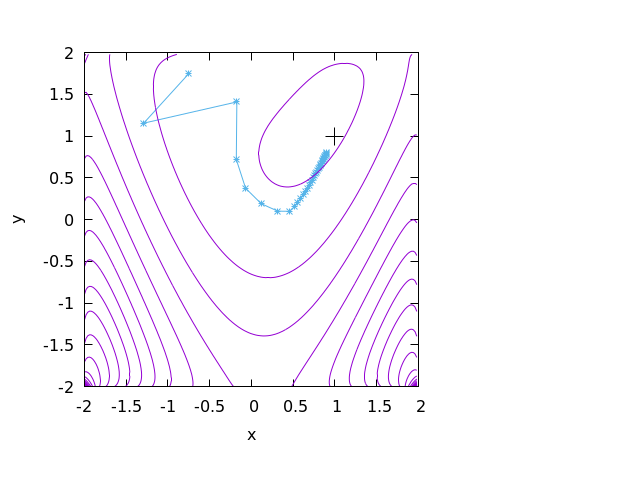
\includegraphics[height=0.5\linewidth]{eps1.png}
	\caption{Położenia kolejnych przybliżeń minimum funkcji $ f(x, y) $ w poszczególnych iteracjach dla $\epsilon = 10^{-2} $. Program wykonał 37 iteracji.}
	\label{pierwszy} 
	\end{center}
\end{figure}
\begin{figure}[h!]
	\begin{center}
	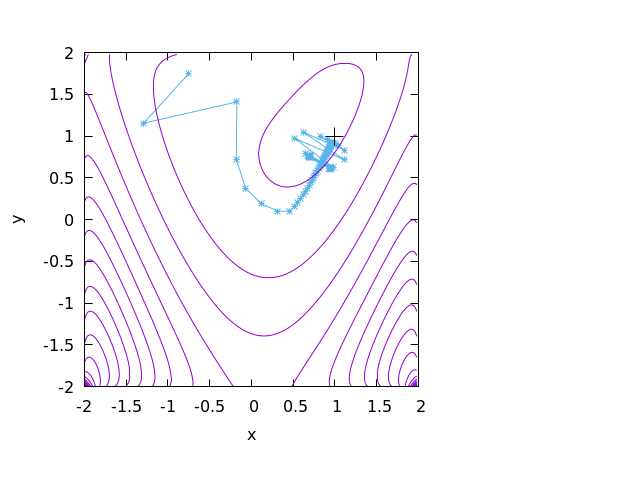
\includegraphics[height=0.5\linewidth]{eps2.png}
	\caption{Położenia kolejnych przybliżeń minimum funkcji $ f(x, y) $ w poszczególnych iteracjach dla $\epsilon = 10^{-3} $. Program wykonał 1000 iteracji.}
	\label{drugi} 
\end{center}
\end{figure}

\newpage
\section{Wnioski}

Wykresy dowodzą, iż ciężko jest wybrać trafne kryterium zbieżności. Dla pierwszego przypadku nie udało się osiągnąć minimum. Zmniejszając rząd zbieżności o jeden, zastosowanie znalazł drugi warunek stopu z uwagi na niekończące się oscylacje wokół poszukiwanego minimum. Potwiedziło to również teoretyczny kształt przebiegu dla funkcji z wydłużonym konturem. Duże znaczenie dla lepszej efektywności uzyskiwanych przybliżeń ma wartość h. Podczas laboratorium skoki nie były regulowane, co znalazło szczególne odbicie w punktach funkcji o niewielkim gradiencie, a w konsekwencji nie osiągnięto zbieżności. Metoda największego spadku może być mało wydajna, jeśli kontur wartości funkcji celu jest wydłużony.
\end{document}